\begin{frame}{Thiết lập xác thực hai lớp (MFA) qua mã QR}
\begin{figure}[H]
\centering
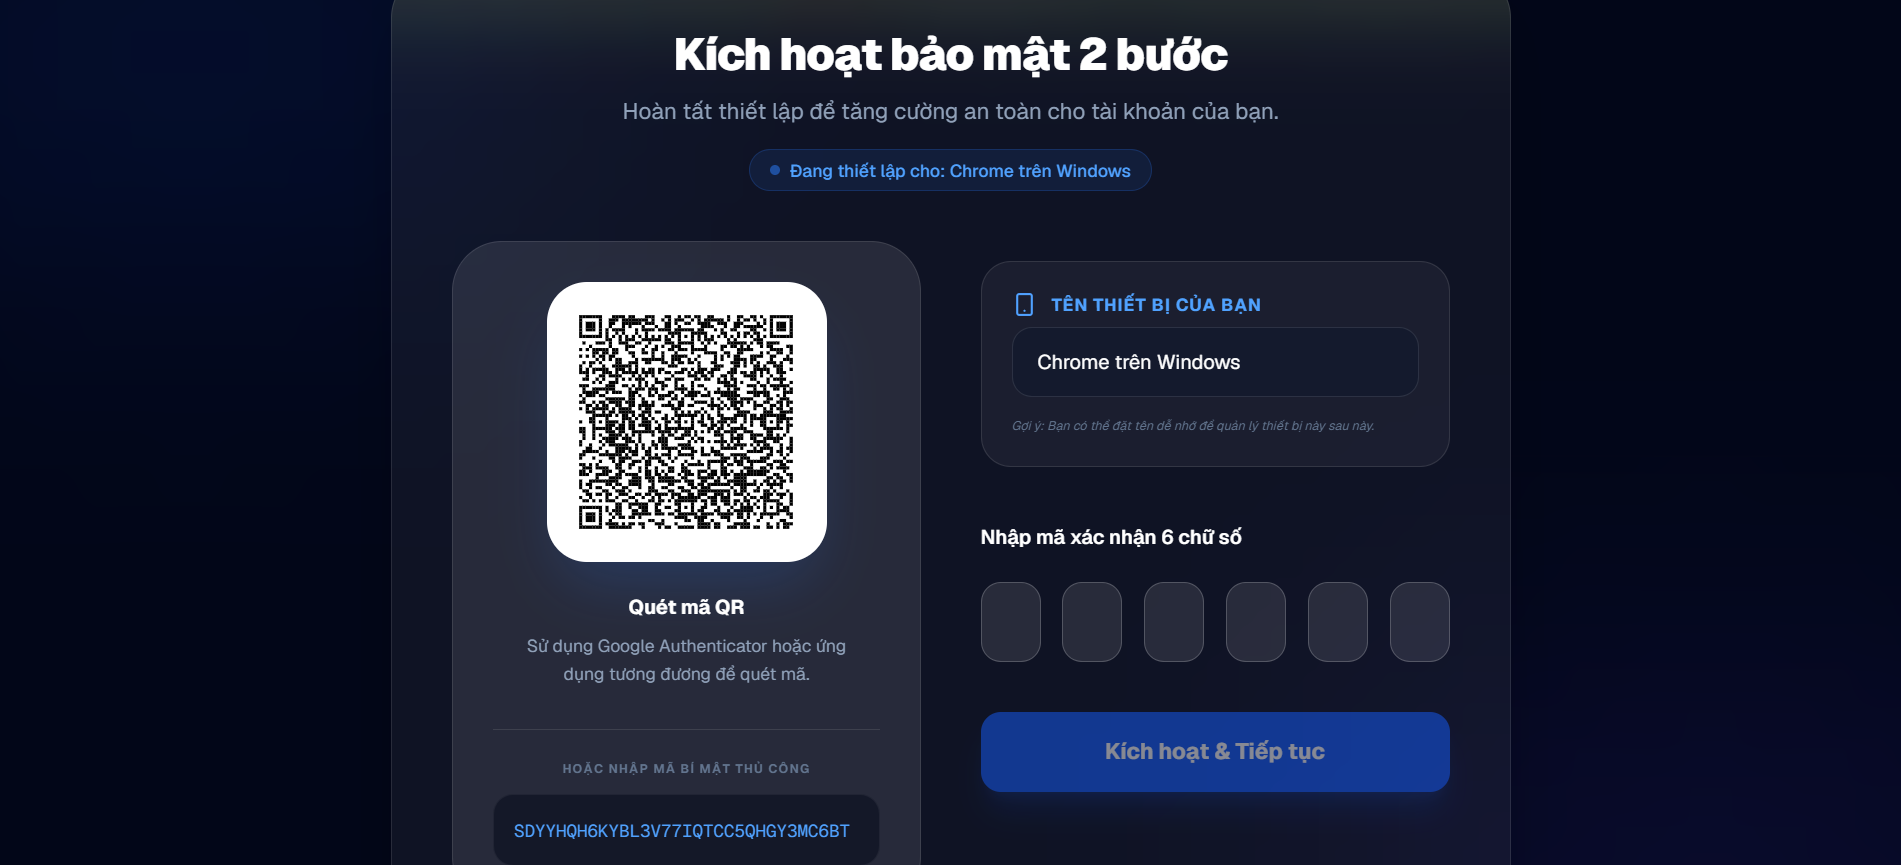
\includegraphics[height=0.55\textheight,width=0.9\textwidth,keepaspectratio]{pictures/WebUI/WebUI-MfaQrSetup.png}
\caption{Kết quả thiết lập MFA bằng mã QR}
\end{figure}

\note{
Giao diện thiết lập xác thực đa yếu tố (MFA) trong ứng dụng.
Hệ thống hiển thị một mã QR đại diện cho khóa bí mật được tạo ngẫu nhiên từ máy chủ xác thực. Người dùng sử dụng các ứng dụng Authenticator thông dụng (như Google Authenticator hoặc Microsoft Authenticator) để quét mã QR này nhằm liên kết và lưu trữ khóa bảo mật trên thiết bị di động của họ.
}
\end{frame}
